\documentclass[10pt,t,aspectratio=43,handout]{beamer} % handout aspectratio=149,1610,32,54
\usetheme{Heverlee}
\usepackage{amsmath,amssymb}
\usepackage{tikz-cd,tikz}
\usepackage{mathtools,mathbbol}
\usepackage{subcaption}
% environments
%\newtheorem{theorem}{Theorem}
%\newtheorem{proposition}[theorem]{Proposition}
%\newtheorem{lemma}[theorem]{Lemma}
%\newtheorem{corollary}[theorem]{Corollary}
%
%\theoremstyle{definition}
%\newtheorem{definition}[theorem]{Definition}
%\newtheorem*{definition*}{Definition}
%\newtheorem{remark}[theorem]{Remark}
%\newtheorem*{remark*}{Remark}
%\newtheorem{example}[theorem]{Example}
%\newtheorem*{example*}{Example}
%\newtheorem{convention}[theorem]{Convention}
%\newtheorem*{convention*}{Convention}
%\newtheorem{notation}[theorem]{Notation}
%\newtheorem*{notation*}{Notation}
%\newtheorem{question}[theorem]{Question}
%\newtheorem*{question*}{Question}

% hyphenation
\hyphenation{co-chain}
\hyphenation{co-chains}
\hyphenation{co-al-ge-bra}
\hyphenation{co-al-ge-bras}
\hyphenation{co-bound-ary}
\hyphenation{co-bound-aries}

% basics
\DeclareMathOperator{\face}{d}
\DeclareMathOperator{\dege}{s}
\DeclareMathOperator{\bd}{\partial}
\DeclareMathOperator{\sign}{sign}
\newcommand{\ot}{\otimes}
\DeclareMathOperator{\EZ}{EZ}
\DeclareMathOperator{\AW}{AW}
\newcommand{\diag}{\mathrm{D}}


% sets and spaces
\newcommand{\N}{\mathbb{N}}
\newcommand{\Z}{\mathbb{Z}}
\newcommand{\Q}{\mathbb{Q}}
\newcommand{\R}{\mathbb{R}}
\renewcommand{\k}{\Bbbk}
\newcommand{\Sym}{\mathbb{S}}
\newcommand{\Cyc}{\mathbb{C}}
\newcommand{\Ftwo}{{\mathbb{F}_2}}
\newcommand{\Fp}{{\mathbb{F}_p}}
\newcommand{\Cp}{{\mathbb{C}_p}}
\newcommand{\gsimplex}{\mathbb{\Delta}}
\newcommand{\gcube}{\mathbb{I}}

% categories
\newcommand{\Cat}{\mathsf{Cat}}
\newcommand{\Fun}{\mathsf{Fun}}
\newcommand{\Set}{\mathsf{Set}}
\newcommand{\Top}{\mathsf{Top}}
\newcommand{\CW}{\mathsf{CW}}
\newcommand{\Ch}{\mathsf{Ch}}
\newcommand{\simplex}{\triangle}
\newcommand{\sSet}{\mathsf{sSet}}
\newcommand{\cube}{\square}
\newcommand{\cSet}{\mathsf{cSet}}
\newcommand{\Alg}{\mathsf{Alg}}
\newcommand{\coAlg}{\mathsf{coAlg}}
\newcommand{\biAlg}{\mathsf{biAlg}}
\newcommand{\sGrp}{\mathsf{sGrp}}
\newcommand{\Mon}{\mathsf{Mon}}
\newcommand{\SymMod}{\mathsf{Mod}_{\Sym}}
\newcommand{\SymBimod}{\mathsf{biMod}_{\Sym}}
\newcommand{\operads}{\mathsf{Oper}}
\newcommand{\props}{\mathsf{Prop}}

% operators
\DeclareMathOperator{\free}{F}
\DeclareMathOperator{\forget}{U}
\DeclareMathOperator{\yoneda}{\mathcal{Y}}
\DeclareMathOperator{\Sing}{Sing}
\newcommand{\loops}{\Omega}
\DeclareMathOperator{\cobar}{\mathbf{\Omega}}
\DeclareMathOperator{\proj}{\pi}
\DeclareMathOperator{\incl}{\iota}

% chains
\DeclareMathOperator{\chains}{N}
\DeclareMathOperator{\cochains}{N^{\vee}}
\DeclareMathOperator{\gchains}{C}

% pair delimiters (mathtools)
\DeclarePairedDelimiter\bars{\lvert}{\rvert}
\DeclarePairedDelimiter\norm{\lVert}{\rVert}
\DeclarePairedDelimiter\angles{\langle}{\rangle}
\DeclarePairedDelimiter\set{\{}{\}}

% other
\newcommand{\id}{\mathsf{id}}
\renewcommand{\th}{\mathrm{th}}
\newcommand{\op}{\mathrm{op}}
\DeclareMathOperator*{\colim}{colim}
\DeclareMathOperator{\coker}{coker}
\DeclareMathOperator{\Med}{\mathcal{M}}
\DeclareMathOperator{\UMed}{\forget(\mathcal{M})}
\newcommand{\Hom}{\mathrm{Hom}}
\newcommand{\End}{\mathrm{End}}
\newcommand{\coEnd}{\mathrm{coEnd}}
\newcommand{\biEnd}{\mathrm{biEnd}}
\newcommand{\xla}[1]{\xleftarrow{#1}}
\newcommand{\xra}[1]{\xrightarrow{#1}}
\newcommand{\defeq}{\stackrel{\mathrm{def}}{=}}

% letters
\newcommand{\bk}{\mathbb{k}}
\newcommand{\bC}{\mathbb{C}}
\newcommand{\bF}{\mathbb{F}}

\newcommand{\sA}{\mathsf{A}}
\newcommand{\sB}{\mathsf{B}}
\newcommand{\sC}{\mathsf{C}}

\newcommand{\cA}{\mathcal{A}}
\newcommand{\cB}{\mathcal{B}}
\newcommand{\cC}{\mathcal{C}}
\newcommand{\cD}{\mathcal{D}}
\newcommand{\cE}{\mathcal{E}}

\newcommand{\cL}{\mathcal{L}}
\newcommand{\cM}{\mathcal{M}}
\newcommand{\cN}{\mathcal{N}}
\newcommand{\cO}{\mathcal{O}}
\newcommand{\cP}{\mathcal{P}}

\newcommand{\cW}{\mathcal{W}}
\newcommand{\cX}{\mathcal{X}}
\newcommand{\cY}{\mathcal{Y}}
\newcommand{\cZ}{\mathcal{Z}}

\newcommand{\rB}{\mathrm{B}}
\newcommand{\rD}{\mathrm{D}}
\newcommand{\rE}{\mathrm{E}}
\newcommand{\rH}{\mathrm{H}}
\newcommand{\rP}{\mathrm{P}}
\newcommand{\rS}{\mathrm{S}}
\newcommand{\rW}{\mathrm{W}}

\newcommand{\bbF}{\mathbb{F}}

% comments
\newcommand{\anibal}[1]{\textcolor{blue}{\underline{Anibal}: #1}}


%!TEX root = ../effc_top.tex

\DeclareMathOperator{\Sq}{Sq}
\newcommand{\colorit}[1]{\textcolor{pblue}{#1}}

\newsavebox\precoproduct
\begin{lrbox}{\precoproduct}
	\begin{tikzpicture}[scale=.3]
	\draw (0,0)--(0,.8);
	\draw (0,0)--(.5,-.5);
	\draw (0,0)--(-.5,-.5);
	\end{tikzpicture}
\end{lrbox}
\newcommand{\coproduct}{% <- this 'right of' is inherited; how to avoid?
	\usebox\precoproduct}

\newsavebox\preproduct
\begin{lrbox}{\preproduct}
	\begin{tikzpicture}[scale=.3]
	\draw (0,0)--(0,-.8);
	\draw (0,0)--(.5,.5);
	\draw (0,0)--(-.5,.5);
	\end{tikzpicture}
\end{lrbox}
\newcommand{\product}{% <- this 'right of' is inherited; how to avoid?
	\usebox\preproduct}

%%% QUICK OPTIONS:
% (A) Math font without serifs, enable line below to make math serif:
    \usefonttheme[onlymath]{serif}

% (B) Re-define primary colour by adjusting the RGB values
%    \definecolor{pblue}{RGB}{0,87,183}
    % Ukraine blue = 0,87,183
    % default = 206,125,66

% (C) Title page graphic (optional) --- this is not for the background image, see \usebackgroundtemplate to change that ---
    %\titlegraphic{\includegraphics[height=2.7cm]{example_figure.pdf}}

% (D) Add logo to bottom right-corner (optional)
    \logo{
\includegraphics[height=0.7cm]{aux/logo}\hspace{12pt}\vspace{-4pt}}

% (E) Choose one (or none) of these lines to add footline bar on all frames
    %\setbeamertemplate{footline}[infoline]  % author, title, insitute
    %\setbeamertemplate{footline}[navigation] % dots swhowing progress
    %\setbeamertemplate{footline}[navsym] % navigation symbols

% (F) Widescreen 16:9 ratio
    %\usepackage[orientation=landscape,size=custom,width=16,height=9,scale=0.45,debug]{beamerposter}

%%% TITLE PAGE INFO:

\title{The diagonal of cellular spaces and effective algebro-homotopical constructions}
\subtitle{CUNY Graduate Center}
\author[ammedmar]{Anibal M. Medina-Mardones}
\institute{Universit\'e Sorbonne Paris Nord}
\date{\today}

\begin{document}
	%!TEX root = ../effc_top.tex

{
	\usebackgroundtemplate{ \parbox[b][\paperheight][b]{\paperwidth}{\centering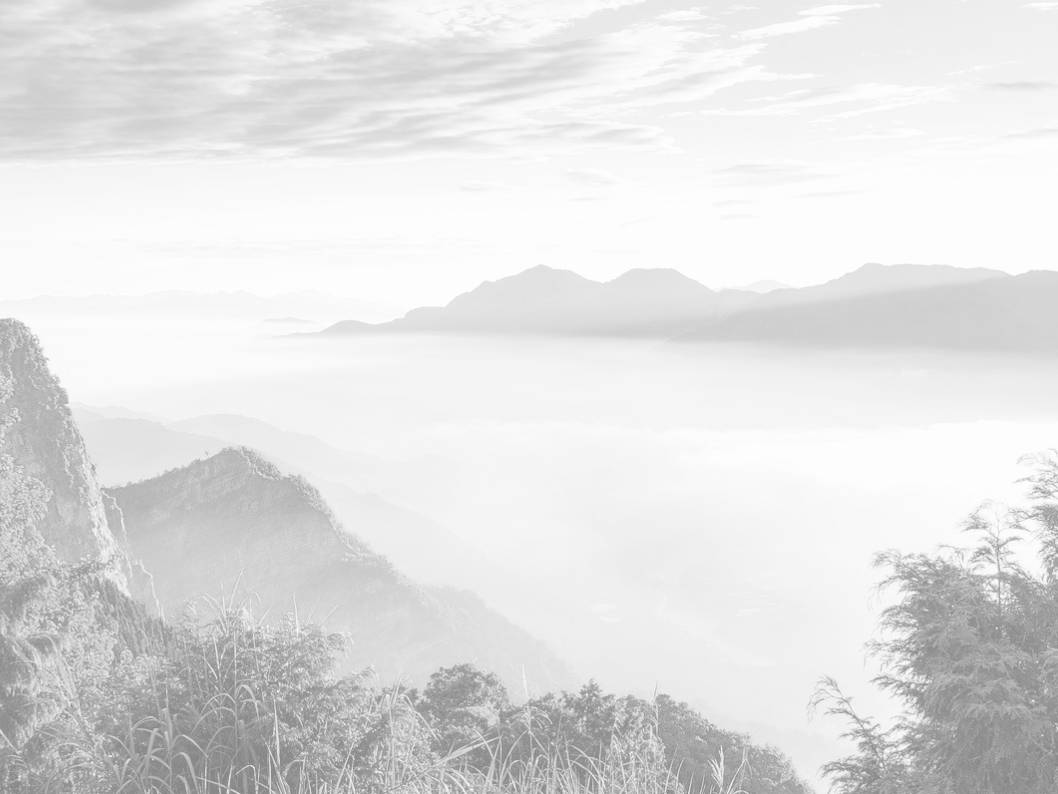
\includegraphics[width=\paperwidth]{aux/background.jpg}}}

	\setbeamercolor{background canvas}{bg=lgray}  % make background light gray

	\begin{frame}[plain,noframenumbering]
	    \titlepage
	\end{frame}
}
	\begin{frame}[plain,noframenumbering]
	\vspace*{2.3cm}
	\begin{center}
		\includegraphics[scale=.2]{aux/ukraine.pdf}
	\end{center}
\end{frame}
	%!TEX root = ../effc_top.tex

\begin{frame}{Viewpoint}
	\vskip -10pt
	\begin{block}{A primary goal of algebraic topology}
		To construct invariants of spaces up to some notion of equivalence.
	\end{block}

	\medskip\pause
	\begin{block}{A basic tension}
		Computability vs. strength of invariants.
	\end{block}

	\medskip \textcolor{pblue}{Example:}
	Homology vs. homotopy.

	\medskip\pause
	\begin{block}{A more subtle tension}
		Effectiveness vs. functoriality of their constructions.
	\end{block}

	\medskip \textcolor{pblue}{Example:}
	cohomology via a cochain complex or \\
	\hspace*{40pt} via maps to Eilenberg-Maclane spaces.
\end{frame}

\begin{frame}{Modeling spaces combinatorially}
	\pause
	\begin{block}{Poincar\'{e}}
		Break spaces into contractible combinatorial pieces: simplices, cubes, ...
	\end{block}

	\pause \textcolor{pblue}{Cohomology:}
	via a cochain complex generated by these pieces.

	\medskip\pause	More generally:
	\begin{block}{Kan-Quillen}
		Use category theory to replace spaces by functors with a geometric realization: simplicial sets, cubical sets, ...
	\end{block}

	\pause \textcolor{pblue}{Basic objects:}
	Chains on standard pieces $\gchains(\gsimplex^n)$, $\gchains(\gcube^n)$, ...

	\smallskip\pause
	\begin{block}{Our goal (loosly stated)}
		Understand these chain complexes deeply to enhance (co)homology with finer effectively computable invariants.
	\end{block}
\end{frame}

\begin{frame}{Shortcomings of (co)homology}
	\pause With mod 2 coefficients the real projective plane and the wedge of a sphere and a circle are isomorphic
	\[
	H^\bullet(\R \rP^2; \Ftwo) \cong H^\bullet(S^1 \vee S^2; \Ftwo)
	\]
	as graded vector spaces.

	\bigskip\pause
	Similarly,
	\[
	H^\bullet(\bC \rP^2; \Z) \cong H^\bullet(S^2 \vee S^4; \Z)
	\]
	as graded abelian groups.

	\bigskip\pause
	\begin{block}{Cup product}
		These can be distinguished by the product in cohomology.
	\end{block}
\end{frame}
	%!TEX root = ../effc_top.tex

\begin{frame}{Shortcomings of cohomology I}
	\pause
	As graded vector spaces
	\[
	H^\bullet(\R \rP^2; \Ftwo) \cong H^\bullet(S^1 \vee S^2; \Ftwo).
	\]

	\pause
	Similarly, as graded abelian groups
	\[
	H^\bullet(\bC \rP^2; \Z) \cong H^\bullet(S^2 \vee S^4; \Z).
	\]

	\pause
	These can be distinguished by the \colorit{product structure} in $H^\bullet$.

	\bigskip\pause
	Defined by dualizing an \textbf{explicit} chain approximation to the diagonal
	\[
	\gchains(\gsimplex^n) \to \gchains(\gsimplex^n) \otimes \gchains(\gsimplex^n)
	\]
	due to Alexander and Whitney.

	\medskip\pause
	Similarly, Cartan and Serre constructed
	\[
	\gchains(\gcube^n) \to \gchains(\gcube^n) \otimes \gchains(\gcube^n).
	\]
\end{frame}

\begin{frame}[fragile]{Shortcomings of cohomology II}
	\pause
	Let $\Sigma$ denotes suspension, for example $\Sigma(S^1)$ is
	\begin{center}
		\includegraphics[scale=.25]{aux/suspension.pdf}
	\end{center}

	\pause\vskip-10pt
	As graded rings
	\[
	H^\bullet(\Sigma(\bC \rP^2)) \cong H^\bullet(\Sigma(S^2 \vee S^4)).
	\]

	\pause
	These can be distinguished by the action of the Steenrod algebra on $H^\bullet$.

	\bigskip\pause
	From the spectral viewpoint this structure is present by definition.

	\bigskip\pause
	\colorit{Question}: Can it be described \textbf{explicitly} at the chain level?
\end{frame}
	%!TEX root = ../effc_top.tex

\begin{frame}[fragile]{Cup product}
	\pause Alexander and Whitney defined the cup product by dualizing a chain approximation to the diagonal:
	\[
	\gchains(\gsimplex^n) \to \gchains(\gsimplex^n) \otimes \gchains(\gsimplex^n).
	\]
	\pause Similarly, Cartan and Serre constructed: $\gchains(\gcube^n) \to \gchains(\gcube^n) \otimes \gchains(\gcube^n)$.

	\bigskip\pause
	As mentioned before, as graded rings,
	\[
	H^\bullet(\bC \rP^2) \not\cong H^\bullet(S^2 \vee S^4).
	\]

	\vskip -8pt \pause But,
	\[
	H^\bullet(\Sigma(\bC \rP^2)) \cong H^\bullet(\Sigma(S^2 \vee S^4)),
	\]
	where $\Sigma$ denotes suspension, for example $\Sigma(S^1)$ is
	\begin{center}
		\includegraphics[scale=.2]{aux/suspension.pdf}
	\end{center}
\end{frame}

\begin{frame}{Steenrod squares}
	\pause These chain approximations, unlike the diagonal of spaces, are \textcolor{pblue}{not} invariant under transposition: $x \otimes y \stackrel{T}{\mapsto} y \otimes x$.
	\begin{center}
		\begin{tikzpicture}
		\draw[color=pblue, thick] (0,0)--(1,1);
		\draw[->] (1.25, .5) -- (1.75, .5);
		\end{tikzpicture}
		\begin{tikzpicture}
		\node at (-0.1, 1){};
		\draw[color=pblue, thick] (0,0)--(1,0)--(1,1);
		\draw (1,1)--(0,1)--(0,0);
		\end{tikzpicture}
	\end{center}

	\smallskip\pause To correct homotopically the breaking of this symmetry, Steenrod introduced explicit maps
	\[
	\Delta_i \colon \gchains(\gsimplex^n) \to \gchains(\gsimplex^n)^{\otimes 2}
	\quad \text{satisfying} \quad
	\partial \Delta_{i} = \big(1 \pm T \big) \Delta_{i-1}
	\]

	\pause

	These induce further structure:
	\[
	\begin{split}
		Sq^k \colon H^\bullet(X; \Ftwo) &\to H^\bullet(X; \Ftwo) \\
		[\alpha] &\mapsto \big[ (\alpha \otimes \alpha) \Delta_i(-) \big]
	\end{split}
	\]

	\vskip-8pt\pause

	\textcolor{pblue}{Distinguishes}
	\[
	H^\bullet(\Sigma(\bC \rP^2)) \not\cong H^\bullet(\Sigma(S^2 \vee S^4))
	\]
\end{frame}

\begin{frame}[fragile]{A (new) description of Steenrod's construction}
	\pause\vskip-5pt
	\textcolor{pblue}{Notation:}
	\vspace*{-5pt}
	\[
	d_u[v_0, \dots, v_m] = [v_0, \dots, \widehat v_u, \dots, v_m]
	\]
	\pause\vspace*{-15pt}
	\[
	\rP_q^n = \set[\big]{U \subseteq \{0, \dots, n\} : \bars{U} = q}
	\]
	\pause\vspace*{-15pt}
	\[
	\forall \, U = \{u_1 < \dots < u_q\} \in \rP_q^n
	\]
	\pause\vspace*{-15pt}
	\[
	d_U = d_{u_1} \dotsm \, d_{u_q}
	\]
	\pause\vspace*{-15pt}
	\[
	U^\varepsilon = \big\{ u_i \in U \mid u_i + i \equiv \varepsilon \text{ mod } 2 \big\}
	\]

	\bigskip\pause
	\textcolor{pblue}{Definition (Med.)} \\
	For a basis element $x \in \gchains_m(\gsimplex^n)$
	\vspace*{-5pt}
	\[
	\Delta_i(x) \ = \!\!\! \sum_{U \in \rP_{m-i}^n} \!\! d_{U^0}(x) \otimes d_{U^1}(x)
	\]
	\vspace*{-10pt}

	\pause
	\textcolor{pblue}{Example:}
	\vspace*{-5pt}
	\begin{align*}
	\Delta_0 [0,1,2] &=
	\Big( d_{12} \otimes \id + d_2 \otimes d_0 + \id \otimes d_{01} \Big) [0,1,2]^{\otimes 2} \\ &=
	[0] \otimes [0,1,2] + [0,1] \otimes [1,2] + [0,1,2] \otimes [2].
	\end{align*}
\end{frame}

\begin{frame}{Fast computation of Steenrod squares}
	\pause
	Comparing with SAGE: (algorithm based on EZ-AW contraction)

	\smallskip\pause
	\textcolor{pblue}{$Sq^1$} on \textcolor{pblue}{$\Sigma^i\R P^2$} ($i^\th$ suspension of the real projective plane)
	\medskip
	\includegraphics[width=\textwidth]{aux/comp_sus_rp2.pdf}
\end{frame}

\begin{frame}[fragile]{Steenrod barcodes}
	\pause
	Given a filtered simplicial complex $X$
	\[
	X_0 \to X_1 \to \cdots \to X_n.
	\]

	\pause
	Cohomology induces a \textcolor{pblue}{persistent module}, its \textcolor{pblue}{barcode} is a summary of how Betti numbers are shared.
	\phantom{$Sq^k$ induces an endomorphism}
	\[
	\begin{tikzcd}[column sep = 15]
		H^\bullet(X_n; \Ftwo) \arrow[r] & \cdots \arrow[r] & H^\bullet(X_{n-1}; \Ftwo) \arrow[r] & \,H^\bullet(X_0; \Ftwo) \phantom{.}
	\end{tikzcd}
	\]
\end{frame}

\begin{frame}[fragile]{Steenrod barcodes}
	Given a filtered simplicial complex $X$
	\[
	X_0 \to X_1 \to \cdots \to X_n.
	\]
	Cohomology induces a \textcolor{pblue}{persistent module}, its \textcolor{pblue}{barcode} is a summary of how Betti numbers are shared.
	$Sq^k$ induces an endomorphism
	\[
	\begin{tikzcd}[column sep = 15]
	H^\bullet(X_n; \Ftwo) \arrow[r] & \cdots \arrow[r] & H^\bullet(X_{n-1}; \Ftwo) \arrow[r] & H^\bullet(X_0; \Ftwo) \\
	H^\bullet(X_n; \Ftwo) \arrow[u, "Sq^k"] \arrow[r] & \cdots \arrow[r] & H^\bullet(X_{n-1}; \Ftwo) \arrow[u, "Sq^k"] \arrow[r] & H^\bullet(X_0; \Ftwo) \arrow[u, "Sq^k"].
	\end{tikzcd}
	\]

	\pause
	The \textcolor{pblue}{$Sq^k$-barcode} of $X$ is the barcode of $\mathrm{img}\ Sq^k$.

	\bigskip\pause
	With \textit{Umberto Lupo} and \textit{Guillaume Tauzin} from \textcolor{pblue}{\texttt{giotto-tda}}'s team
	\medskip
	develop a high-performance implementation: \textcolor{pblue}{\texttt{steenroder}}.
\end{frame}

%\begin{frame}{Comparing persistent $Sq^2$-modules} \pause
%	Filtrations of the cone on the suspension of $S^2 \vee S^4$ and $\bC \rP^2$.
%
%	\pause
%	\begin{figure}
%		\centering
%		\begin{subfigure}[b]{0.49\textwidth}
%			\centering
%			\includegraphics[width=\textwidth]{aux/s2_s4.pdf}
%			\caption{$\mathrm C\,\Sigma(S^2 \vee S^4)$}
%			\label{f:s2_s4}
%		\end{subfigure}
%		\begin{subfigure}[b]{0.49\textwidth}
%			\centering
%			\includegraphics[width=\textwidth]{aux/cp2.pdf}
%			\caption{$\mathrm C\,\Sigma\,\bC\rP^2$}
%			\label{f:cp2}
%		\end{subfigure}
%	\end{figure}
%\end{frame}

\begin{frame}{Space of conformations of $\mathrm{C_8H_{16}}$}
	Points in $\R^{24}$ (positions of $8$ carbons in $\R^3$)

	\pause\smallskip
	Computing $Sq^1$ barcode of a ``smooth component'' of this point cloud
	\smallskip
	\includegraphics[width=\textwidth]{aux/cyclo-octane_subsampled_absolute_barcodes.pdf}
	Consistent with a \textcolor{pblue}{Klein bottle} component.
\end{frame}

\begin{frame}{More on cup-$i$ constructions}
	\pause
	\textcolor{pblue}{Theorem (Med.)} \\
	All cup-$i$ constructions in the literature are equal up isomorphism:
	\[
	\triangle \sim \triangle^\prime \iff \forall i \in \N, \ \triangle_i = \triangle_i^\prime \ \vee \, \triangle_i = T \triangle_i^\prime.
	\]
	(Proven via an axiomatic characterization.)

	\bigskip\pause
	\textcolor{pblue}{Theorem (Med.)} \\
	Steenrod's cup-$i$ construction defines the nerve of higher categories.

	\bigskip\pause
	\textcolor{pblue}{Theorem (Laplante-Anfossi--Med.--Vallette)} \\
	Let $P \subset \R^n$ be an $n$-dim convex polytope.
	A generic basis of $\R^n$ defines a cellular cup-$i$ construction $S^\infty \times P \to P \times P$.

	\bigskip\pause
	\textcolor{pblue}{Theorem (Cantero-Mor\'an)} \\
	Interpretation of these formulas for Khovanov homology.
\end{frame}

\begin{frame}{Relations}
	\pause
	There are two main Steenrod square relations:

	\bigskip\pause
	\textcolor{pblue}{Cartan}
	\vspace*{-5pt}
	\begin{equation*}
		Sq^k \big( [\alpha] [\beta] \big) =
		\sum_{i+j=k} \, Sq^i\big([\alpha]\big) Sq^j\big([\beta]\big),
	\end{equation*}

	\pause
	\textcolor{pblue}{Adem}
	\vspace*{-5pt}
	\begin{equation*}
		Sq^i Sq^j =
		\sum_{k=0}^{\lfloor i/2 \rfloor} \binom{j-k-1}{i-2k} Sq^{i+j-k} Sq^k.
	\end{equation*}

	\medskip\pause
	\textcolor{pblue}{Construction (Brumfiel--Med.--Morgan)} \\
	Explicit cochains witnessing these relations at the cochain level.

	\medskip\pause
	\textcolor{pblue}{Application (Gaiotto, Kapustin, Thorngren and others)} \\
	Used these in the classification of topological phases.

	\medskip\pause
	\textcolor{pblue}{Vague idea} \\
	Cochains as fields on triangulated spacetime with actions using these.
\end{frame}
	%!TEX root = ../effc_top.tex

\begin{frame}[fragile]{Operations at odd primes}
	\pause
	Steenrod squares come from the symmetry of the \textbf{binary} diagonal.

	\medskip\pause
	Steenrod, and more generally May, also defined operations
	\[
	P_k \colon H^\bullet(X; \Fp) \to H^\bullet(X; \Fp)
	\]
	from the symmetry of $X \to X \times \dots \times X$.

	\medskip\pause
	\colorit{Note}: indirect group homology definition.
	No generalizations of cup-$i$.

	\bigskip\pause
	\colorit{Construction (Kaufmann-Med.)} \\
	Explicit cup-$(p,i)$ products defining these operations.

	\medskip\pause
	\colorit{Example} \\
	Using the computer algebra system \colorit{\texttt{ComCH}} we have $\Delta_{3,2}[0,1,2] = $

	\begin{verbatim}
		- [0,1][0,1,2][0,1] + [0,1,2][0,2][0,1] + [0,2][0,2][0,1,2]
		- [0,1,2][0,1,2][1] - [0,2][0,1,2][1,2] + [0,1,2][1,2][1,2]
		- [0,1][1,2][0,1,2] - [0,1,2][2][0,1,2] - [0][0,1,2][0,1,2]
	\end{verbatim}
\end{frame}

\begin{frame}{A more abstract viewpoint}
	\pause
	Operads control algebraic structures.

	\bigskip\pause
	The operad $\mathcal{C}om$ controls cocommutative and coassociative coalgebras.

	\bigskip\pause
	An $E_\infty$-operad is an $\Sym$-cofibrant resolution of $\mathcal{C}om$.

%	\bigskip\pause
%	$E_\infty$-structures have a long history:
%	\smallskip\pause
%	\begin{itemize}
%		\item (co)homology operations,
%		\item recognition of infinite loop spaces,
%		\item algebraic models of the homotopy category.
%	\end{itemize}

	\bigskip\pause
	\colorit{Fact}:
	The chains of a space can be made into an $E_\infty$-coalgebra by fully deriving the diagonal map.

	\bigskip\pause
	\colorit{Principle} (Quillen, Sullivan, Mandell, ...) \\
	\textbf{All} homotopy information of spaces is in this algebraic model.

	\bigskip\pause
	\colorit{Question}: How explicit can this $E_\infty$-structure be?

	\bigskip\pause
	Constructions by McClure--Smith and Berger--Fresse generalized by:
\end{frame}

\begin{frame}{Explicit $E_\infty$-structure on (co)chains}

	\colorit{Theorem (Med.)} \\
	The collection of maps $\gchains(\gsimplex^n) \to \gchains(\gsimplex^n)^{\otimes r}$ obtained from compositions of
	\begin{align*}
		\Delta &\colon \gchains(\gsimplex^n) \to \gchains(\gsimplex^n)^{\otimes 2}
		\qquad \text{(AW diagonal)} \\
		\ast &\colon \gchains(\gsimplex^n)^{\otimes 2} \to \gchains(\gsimplex^n)
		\qquad \text{(Join map)}
	\end{align*}
	defines an $E_\infty$-coalgebra on simplicial chains.

	\bigskip\pause
	\colorit{Join map} \\
	\qquad\qquad \scalebox{0.7}{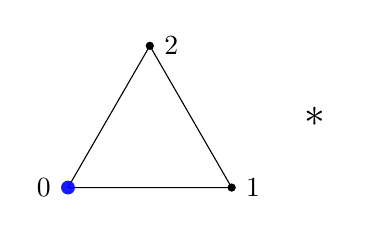
\begin{tikzpicture}[scale=.6]
\coordinate (A) at (210:2);
\coordinate (B) at (-30:2);
\coordinate (C) at (90:2);

\draw[draw=black] (A) -- (B) -- (C) -- (A);

\node[circle,fill=blue, opacity=.9, inner sep=0pt,minimum size=5pt, label=left:{0}] (a) at (A) {};
\node[circle,fill=black,inner sep=0pt,minimum size=3pt, label=right:{$1$}] (a) at (B) {};
\node[circle,fill=black,inner sep=0pt,minimum size=3pt, label=right:{$2$}] (a) at (C) {};

\node[scale=1.5] at (3.5,0.5) {$\ast$};
\end{tikzpicture}
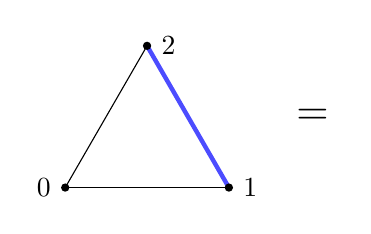
\begin{tikzpicture}[scale=.6]
\coordinate (A) at (210:2);
\coordinate (B) at (-30:2);
\coordinate (C) at (90:2);

\draw[draw=blue,  ultra thick, draw opacity=.7] (B) -- (C);
\draw[draw=black] (C) -- (A);
\draw[draw=black] (A) -- (B);

\node[circle,fill=black,inner sep=0pt,minimum size=3pt, label=left:{$0$}] (a) at (A) {};
\node[circle,fill=black,inner sep=0pt,minimum size=3pt, label=right:{$1$}] (a) at (B) {};
\node[circle,fill=black,inner sep=0pt,minimum size=3pt, label=right:{$2$}] (a) at (C) {};

\node[scale=1.5] at (3.5,.5) {=};
\end{tikzpicture}
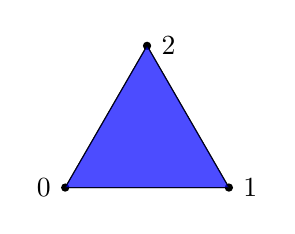
\begin{tikzpicture}[scale=.6]
\coordinate (A) at (210:2);
\coordinate (B) at (-30:2);
\coordinate (C) at (90:2);

\draw[draw=black] (A) -- (B) -- (C) -- (A);

\node[circle,fill=black,inner sep=0pt,minimum size=3pt, label=left:{$0$}] (a) at (A) {};
\node[circle,fill=black,inner sep=0pt,minimum size=3pt, label=right:{$1$}] (a) at (B) {};
\node[circle,fill=black,inner sep=0pt,minimum size=3pt, label=right:{$2$}] (a) at (C) {};

\draw[draw, fill=blue, opacity=.7] (A) -- (B) -- (C) -- (A);
\end{tikzpicture}}

	\bigskip\pause
	\colorit{Other versions} \\
	\colorit{1)} Cubical (Kaufmann--Med.) \\
	\colorit{2)} Multisimplicial (Med.--Pizzi--Salvatore).
\end{frame}

\begin{frame}{A finitely presented $E_\infty$-prop}
	\pause Consider the prop $\cM$ generated by
	\[
	\begin{tikzpicture}[scale=.4]
		\draw (0,.5)--(0,-.75);
		\node[scale=.5] at (0,.75){1};
		\fill (0,-.65) circle (3pt);
	\end{tikzpicture}
	\qquad
	\begin{tikzpicture}[scale=.4]
		\draw (0,0)--(0,.75);
		\draw (0,0)--(.5,-.5);
		\draw (0,0)--(-.5,-.5);
		\node[scale=.5] at (-.5,-.75){1};
		\node[scale=.5] at (.5,-.75){2};
	\end{tikzpicture}
	\qquad
	\begin{tikzpicture}[scale=.4]
		\draw (0,0)--(0,-.75);
		\draw (0,0)--(.5,.5);
		\draw (0,0)--(-.5,.5);
		\node[scale=.5] at (-.5,.75){1};
		\node[scale=.5] at (.5,.75){2};
	\end{tikzpicture}
	\vspace*{-2pt}
	\]
	in degrees $0, 0$ \& $1$ with non-zero boundary
	\[
	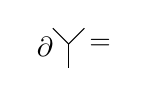
\begin{tikzpicture}[scale=.4]
		\node[scale=1] at (-.75,-.1){$\partial$};
		\draw (0,0)--(0,-.75);
		\draw (0,0)--(.5,.5);
		\draw (0,0)--(-.5,.5);
		\node[scale=1] at (1,0){$=$};
	\end{tikzpicture}
	\begin{tikzpicture}[scale=.4]
		\draw (0,.5)--(0,-.75);
		\fill (0,-.65) circle (3pt);
		\draw (.5,.5)--(.5,-.75);
		\node[scale=1] at (1.15,0){$-$};
	\end{tikzpicture}
	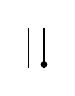
\begin{tikzpicture}[scale=.4]
		\draw (0,.5)--(0,-.75);
		\fill (.5,-.65) circle (3pt);
		\draw (.5,.5)--(.5,-.75);
	\end{tikzpicture}
	\]
	\vskip-5pt
	and relators
	\[
	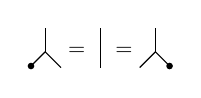
\begin{tikzpicture}[scale=.4]
		\draw (0,0)--(0,.75);
		\draw (0,0)--(.5,-.5);
		\draw (0,0)--(-.5,-.5);
		\fill (-.45,-.45) circle (3pt);
		\node[scale=.8] at (1,0){$=$};
		\draw (1.75,.75)--(1.75,-.5);
		\node[scale=.8] at (2.5,0){$=$};
		\draw (3.5,0)--(3.5,.75);
		\draw (3.5,0)--(4,-.5);
		\draw (3.5,0)--(3,-.5);
		\fill (3.95,-.45) circle (3pt);
	\end{tikzpicture}
	\quad\qquad
	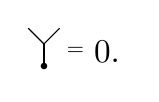
\begin{tikzpicture}[scale=.4]
		\draw (0,0)--(0,-.75);
		\draw (0,0)--(.5,.5);
		\draw (0,0)--(-.5,.5);
		\fill (0,-.7) circle (3pt);
		\node[scale=.8] at (1,-.25){$=$};
		\node[scale=1.2] at (2,-.25){$0.$};
	\end{tikzpicture}
	\]

	\medskip\pause
	\colorit{Theorem (Med.)} \\
	The operad associated to $\Med$, defined by
	\[
	\forget(\cM) = \{\cM(1,r)\}_{r \geq 1},
	\]
	is a (cofibrant and Hopf) $E_\infty$-operad.
\end{frame}
	%!TEX root = ../effc_top.tex

\begin{frame}[fragile]{Proof}
	\colorit{Basic case:} $\cM(s,0) \cong \Z\{
	\raisebox{-3pt}{
		\begin{tikzpicture}[scale=.3]
			\draw (0,.5)--(0,-.75);
			\node[scale=.4] at (0,.75){1};
			\fill (0,-.65) circle (3pt);

			\node[scale=.4] at (.55,0){$\dots$};

			\draw (1,.5)--(1,-.75);
			\node[scale=.5] at (1,.75){$s$};
			\fill (1,-.65) circle (3pt);
		\end{tikzpicture}
	}\}$

	\medskip\pause

	\colorit{Contraction:} $\bd \circ \, h = \id - p \circ i + h \circ \bd$
	\vskip -5pt
	\[
	\begin{tikzcd}
		\cM(s,r-1) \arrow[r, "i", shift left=3pt]
		& \cM(s,r) \arrow[l, "p", shift left=3pt] \arrow[loop right, "h", distance=2em]
	\end{tikzcd}
	\]
	\pause\vskip -20pt
	\[
	\begin{tikzpicture}[scale=.3]
		\draw (0,1) -- (0,-1);
		\draw (1,1) -- (1,-1);
		\draw (0,.5) -- (1,.5);
		\draw (0,-.5) -- (1,-.5);
		\node[scale=.4] at (0,1.25){$1$};
		\node[scale=.4] at (0,-1.25){$1$};
		\node[scale=.4] at (1,1.25){$s$};
		\node[scale=.4] at (1,-1.25){$r-1$};
		\draw (1.5,0) edge[|->] (5.5,0);
	\end{tikzpicture}
	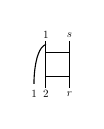
\begin{tikzpicture}[scale=.3]
		\draw (0,1) -- (0,-1);
		\draw (1,1) -- (1,-1);
		\draw (0,.5) -- (1,.5);
		\draw (0,-.5) -- (1,-.5);
		\node[scale=.4] at (0,1.25){$1$};
		\node[scale=.4] at (0,-1.25){$2$};
		\node[scale=.4] at (1,1.25){$s$};
		\node[scale=.4] at (1,-1.25){$r$};
		\draw (0,.85) edge[out=200,in=-90] (-.5,-.7);
		\node[scale=.4] at (-.5,-1.25){$1$};
	\end{tikzpicture}
	\]
	\vskip -10pt
	\[
	\begin{tikzpicture}[scale=.3]
		\node at (-7.5,0){};
		\draw (-5,1) -- (-5,-1);
		\draw (-6,1) -- (-6,-1);
		\draw (-6,.5) -- (-5,.5);
		\draw (-6,-.5) -- (-5,-.5);
		\node[scale=.4] at (-6,1.25){$1$};
		\fill (-6,-.95) circle (3pt);
		\node[scale=.4] at (-5,1.25){$s$};
		\node[scale=.4] at (-5,-1.25){$r-1$};
		\draw (-4.5,0) edge[<-|] (-.5,0);
		%%%%%%%%%%%%%%%%%%%%%%%%%%%%%%%%%
		\draw (0,1) -- (0,-1);
		\draw (1,1) -- (1,-1);
		\draw (0,.5) -- (1,.5);
		\draw (0,-.5) -- (1,-.5);
		\node[scale=.4] at (0,1.25){$1$};
		\node[scale=.4] at (0,-1.25){$1$};
		\node[scale=.4] at (1,1.25){$s$};
		\node[scale=.4] at (1,-1.25){$r$};
		\draw (1.5,0) edge[out=0,in=0,|->] (1.5,-4);
		%%%%%%%%%%%%%%%%%%%%%%%%%%%%%%%%%
		\draw (0,-3) -- (0,-5);
		\draw (1,-3) -- (1,-5);
		\draw (0,-3.5) -- (1,-3.5);
		\draw (0,-4.5) -- (1,-4.5);
		\node[scale=.4] at (0,-2.75){$1$};
		\node[scale=.4] at (0,-5.25){$1$};
		\node[scale=.4] at (1,-2.75){$s$};
		\node[scale=.4] at (1,-5.25){$r$};
		\draw (0,-3.15) edge[out=200,in=160] (0,-4.85);
	\end{tikzpicture}
	\]
	\pause\vskip -25pt\colorit{Then}
	\[
	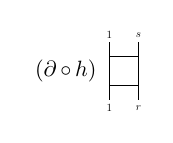
\begin{tikzpicture}[scale=.37]
		\node[scale=.8] at (-1.5,0){$(\bd \circ \, h)$};
		\draw (0,1) -- (0,-1);
		\draw (1,1) -- (1,-1);
		\draw (0,.5) -- (1,.5);
		\draw (0,-.5) -- (1,-.5);
		\node[scale=.4] at (0,1.25){$1$};
		\node[scale=.4] at (0,-1.25){$1$};
		\node[scale=.4] at (1,1.25){$s$};
		\node[scale=.4] at (1,-1.25){$r$};
	\end{tikzpicture}
	\pause
	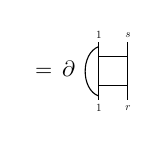
\begin{tikzpicture}[scale=.37]
		\node[scale=.8] at (-1.5,.1){$= \, \bd $};
		\draw (0,1) -- (0,-1);
		\draw (1,1) -- (1,-1);
		\draw (0,.5) -- (1,.5);
		\draw (0,-.5) -- (1,-.5);
		\node[scale=.4] at (0,1.25){$1$};
		\node[scale=.4] at (0,-1.25){$1$};
		\node[scale=.4] at (1,1.25){$s$};
		\node[scale=.4] at (1,-1.25){$r$};
		\draw (0,.85) edge[out=200,in=160] (0,-.85);
	\end{tikzpicture}
	\pause
	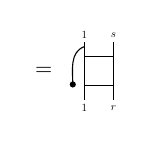
\begin{tikzpicture}[scale=.37]
		\node[scale=.8] at (-1.4,0){$=$};
		\draw (0,1) -- (0,-1);
		\draw (1,1) -- (1,-1);
		\draw (0,.5) -- (1,.5);
		\draw (0,-.5) -- (1,-.5);
		\node[scale=.4] at (0,1.25){$1$};
		\node[scale=.4] at (0,-1.25){$1$};
		\node[scale=.4] at (1,1.25){$s$};
		\node[scale=.4] at (1,-1.25){$r$};
		\draw (0,.85) edge[out=200,in=90] (-.4,-.5);
		\fill (-.4,-.45) circle (3pt);
	\end{tikzpicture}
	\begin{tikzpicture}[scale=.37]
		\node[scale=.8] at (-1.4,0){$\ -$};
		\draw (0,1) -- (0,-1);
		\draw (1,1) -- (1,-1);
		\draw (0,.5) -- (1,.5);
		\draw (0,-.5) -- (1,-.5);
		\node[scale=.4] at (0,1.25){$1$};
		\fill (0,-.95) circle (3pt);
		\node[scale=.4] at (1,1.25){$s$};
		\node[scale=.4] at (1,-1.25){$r$};
		\draw (0,.85) edge[out=200,in=-90] (-.5,-.7);
		\node[scale=.4] at (-.5,-1.25){$1$};
	\end{tikzpicture}
	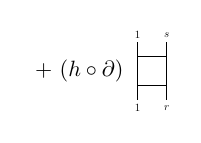
\begin{tikzpicture}[scale=.37]
		\node[scale=.8] at (-2,0){$+\ (h \circ \bd)$};
		\draw (0,1) -- (0,-1);
		\draw (1,1) -- (1,-1);
		\draw (0,.5) -- (1,.5);
		\draw (0,-.5) -- (1,-.5);
		\node[scale=.4] at (0,1.25){$1$};
		\node[scale=.4] at (0,-1.25){$1$};
		\node[scale=.4] at (1,1.25){$s$};
		\node[scale=.4] at (1,-1.25){$r$};
	\end{tikzpicture}
	\pause
	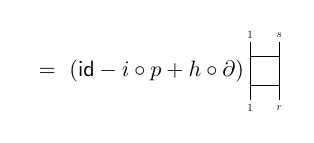
\begin{tikzpicture}[scale=.37]
		\node[scale=.8] at (-3.8,0){$\, = \ (\id - i \circ p + h \circ \bd)$};
		\draw (0,1) -- (0,-1);
		\draw (1,1) -- (1,-1);
		\draw (0,.5) -- (1,.5);
		\draw (0,-.5) -- (1,-.5);
		\node[scale=.4] at (0,1.25){$1$};
		\node[scale=.4] at (0,-1.25){$1$};
		\node[scale=.4] at (1,1.25){$s$};
		\node[scale=.4] at (1,-1.25){$r$};
	\end{tikzpicture}
	\]
\end{frame}
	\begin{frame}[fragile]{Two $E_\infty$-bialgebra models for loop spaces}
	\pause
	\colorit{Construction (Adams)}
	\vspace*{-1pt}
	\begin{center}
		Based space $(X,x)$ \\ \pause
		$\Downarrow$ \\
		Two algebras
		and a q-iso of algebras: \\
		\medskip
		$\mathbb{\Omega} \rS^{\triangle}(X, x)$
		$\xra{\quad \theta_X \quad }$
		$\rS^{\square}(\Omega_x X)$
	\end{center}

	\begin{minipage}{.45\textwidth}
		\begin{flushright}
			Cobar const. on based \\
			simplicial sing. chains
		\end{flushright}
	\end{minipage}
	\hspace*{.9cm}
	\begin{minipage}{.4\textwidth}
		Cubical sing. chains \\
		on based loop space
	\end{minipage}

	\bigskip\smallskip\pause
	\colorit{Theorem (Baues)} \\
	$\theta_X$ is a map of bialgebras.

	\bigskip\pause
	\colorit{Theorem (Med.--Rivera)} \\
	$\theta_X$ is a map of $E_\infty$-bialgebras.

	\bigskip\pause
	The $E_\infty$-coalgebra structure on the domain is defined using an isomorphism $\mathbb{\Omega} \rS^{\triangle}(X, x) \cong \chains^{\cube}(\mathbf{\Omega}_x X)$ where $\mathbf{\Omega}_x X$ is a cubical monoid.
\end{frame}
	%!TEX root = ../effc_top.tex

\begin{frame}{Conclusions and future directions}
	\pause
	\colorit{Slogan} \\
	Homotopy theory requires additional structure to be used ``concretely.'' \\

	\medskip\pause
	\colorit{Today's focus} \\
	The algebro-homotopical diagonal of spaces.

	\medskip\pause
	\colorit{I.}
	\underline{Steenrod cup-$i$ coproducts}

	\medskip\pause
	\colorit{Applications } \\
	Steenrod barcodes, knot invariants, lattice TFTs, L-theory, \\
	higher categories, convex geometry.

	\smallskip\pause
	\colorit{Future} \\
	Incorporate cup-$(p,i)$ coproducts.

	\medskip\pause
	\colorit{II.}
	\underline{Finitely presented prop $\cM$ modeling $E_\infty$}

	\medskip\pause
	\colorit{Application} \\
	Adams cobar as an $E_\infty$-bialgebra model of based loop spaces.

	\smallskip\pause
	\colorit{Future} \\
	Double and free loop spaces.
\end{frame}
	%!TEX root = ../effc_top.tex

{
	\usebackgroundtemplate{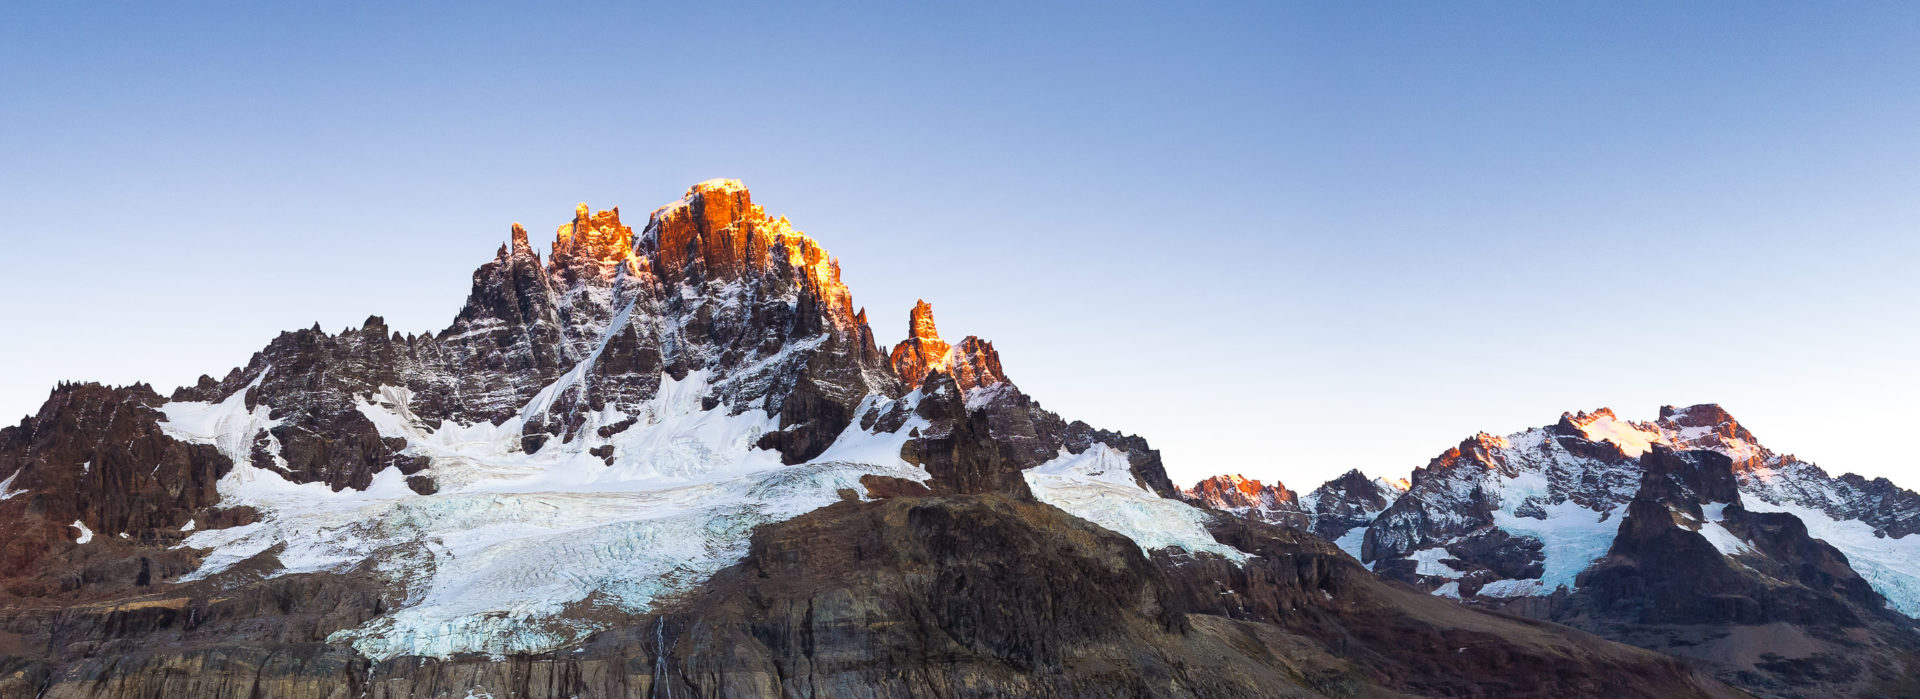
\includegraphics[width=\paperwidth]{aux/castillo.jpg}}%
	\begin{frame}
		\vskip 6cm
		\begin{center}
			\colorit{\Huge Happy Birthday Gunnar!}
		\end{center}
	\end{frame}
}
\end{document}
